\chapter{Precipitación y solubilidad}\label{ch:b1:precipitation}

Una gota de nitrato de plata cae en agua del grifo y aparece una nube
blanca: cloruro de plata, formado a partir de los pocos miligramos de
iones cloruro que contiene cada litro. El agua que se filtra a través de
la caliza arrastra carbonato de calcio y lo vuelve a depositar, una
fracción de milímetro al año, en forma de estalactitas de una cueva. Un
cálculo renal también es un precipitado. Cada uno de estos casos es un
equilibrio entre un sólido y sus iones en disolución, y una sola
constante, el \omterm{def:b1:precipitation:solubility-product}{producto de solubilidad}, dice si el sólido se forma, cuánto
se disuelve y cómo cambia su \omterm{def:b1:precipitation:solubility}{solubilidad} cuando se modifica otro ion o el
pH. Con ella, un químico puede separar unos iones de otros
precipitándolos sucesivamente --- la base del tratamiento de las aguas de
mina con el que termina este capítulo.

\begin{recall}
El volumen escolar (años 6 y 12) midió la \omterm{def:b1:precipitation:solubility}{solubilidad} en gramos por litro
e identificó iones por los precipitados que dan. La constante de
equilibrio, el \omterm{def:b1:extent-q-and-k:quotient}{cociente de reacción} $Q$ y las \omterm{def:b1:extent-q-and-k:activity}{actividades} (1 para un
sólido puro o el disolvente, $c/c^\circ$ para un soluto) se establecieron
en el
\cref{ch:b1:extent-q-and-k}: una reacción avanza mientras $Q < K$. El
método de la \omterm{def:b1:predominant-reaction:predominant-reaction}{reacción predominante} y la escala de $\mathrm{p}K_a$
proceden del
\cref{ch:b1:predominant-reaction}; $c^\circ = \qty{1}{mol/L}$ no se
escribe en los cocientes.
\end{recall}

\begin{omfigure}
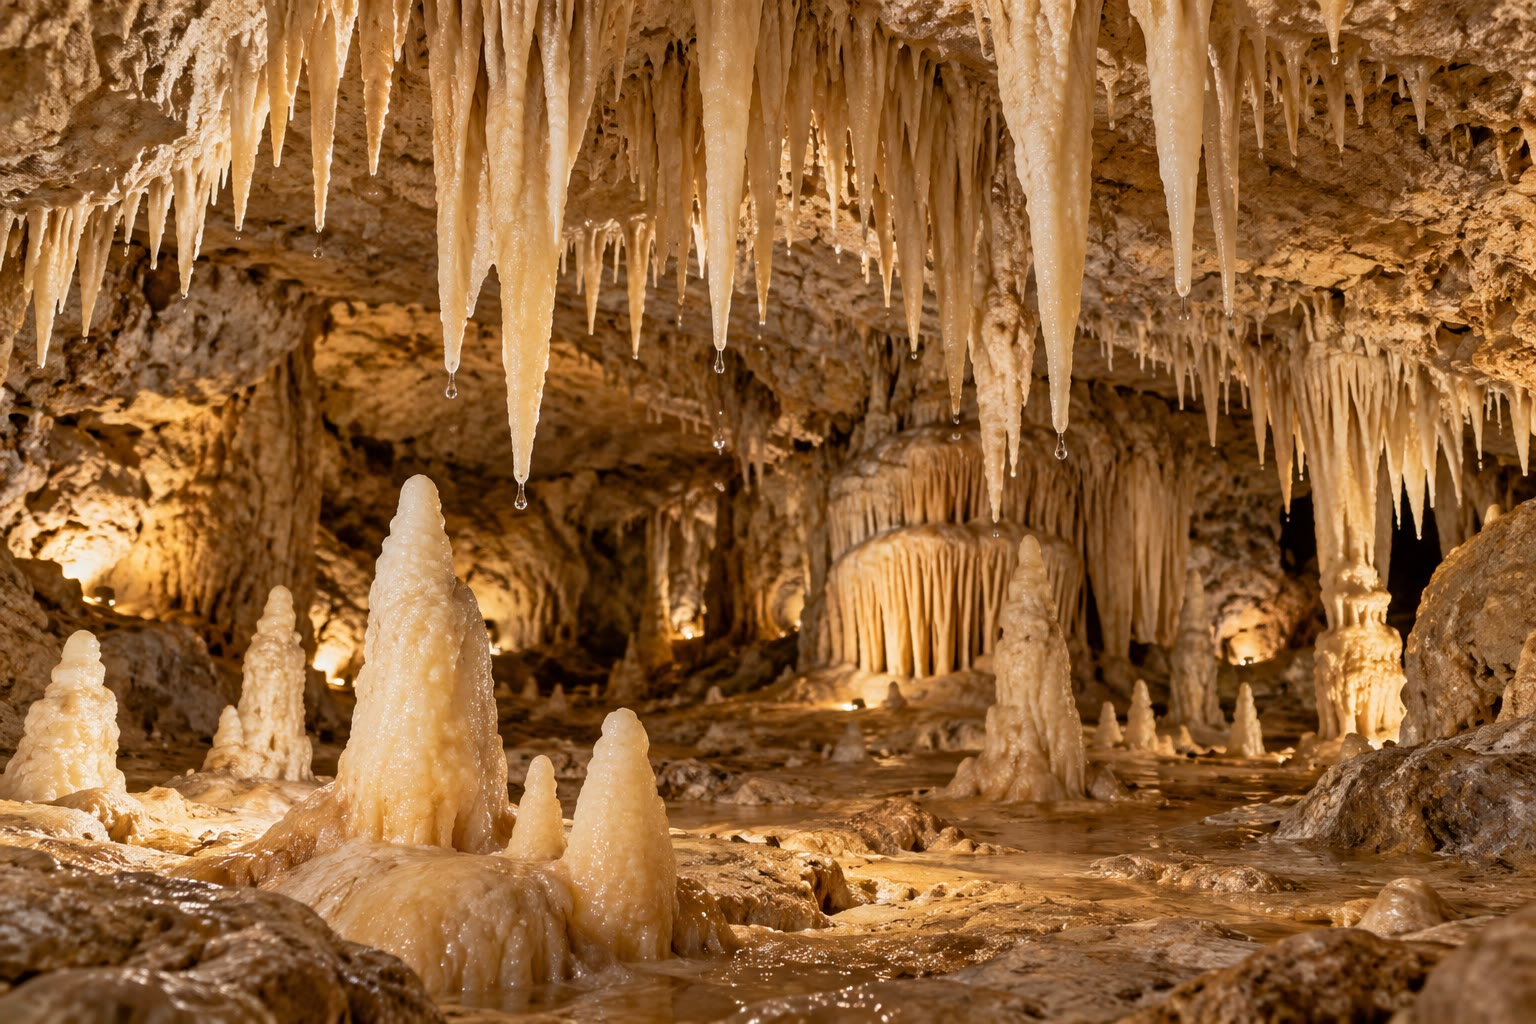
\includegraphics[width=0.62\linewidth]{images/book2/ai/b1-11-cave.jpg}

{\small Estalactitas y estalagmitas en una cueva caliza. El agua rica en
dióxido de carbono disuelve el carbonato de calcio del suelo de encima;
en la cueva pierde parte de su dióxido de carbono y el carbonato vuelve a
precipitar
(\cref{exo:b1:precipitation:10}).}
\end{omfigure}

\section{El producto de solubilidad}\label{sec:b1:precipitation:product}

Un \omterm{def:b1:crystals-metals:crystal}{cristal} de cloruro de plata introducido en agua cede iones a la
disolución, y la disolución devuelve algunos al \omterm{def:b1:crystals-metals:crystal}{cristal}. Cuando las dos
velocidades son iguales, la disolución está \emph{saturada}: su
composición ya no cambia, aunque los iones siguen pasando en los dos
sentidos (figura de abajo).

\begin{definition}[Producto de solubilidad]\label{def:b1:precipitation:solubility-product}
El \emph{producto de solubilidad}\index{producto de solubilidad} $K_s$ de
un sólido iónico $\mathrm{M}_a\mathrm{X}_b$ es la constante de equilibrio
de su disolución en sus iones,
\[
  \mathrm{M}_a\mathrm{X}_b\mathrm{(s)} \rightleftharpoons a\,\mathrm{M}^{m+}
  + b\,\mathrm{X}^{x-}, \qquad
  K_s = [\mathrm{M}^{m+}]_{\mathrm{eq}}^{\,a}\,[\mathrm{X}^{x-}]_{\mathrm{eq}}^{\,b},
  \qquad \mathrm{p}K_s = -\log K_s ,
\]
pues la \omterm{def:b1:extent-q-and-k:activity}{actividad} del sólido es 1. Como toda constante de equilibrio,
solo depende de la temperatura.
\end{definition}

Para el cloruro de plata, \ce{AgCl(s) <=> Ag+ + Cl-} y $K_s =
[\ce{Ag+}][\ce{Cl-}] = 10^{-9.75}$; para el fluoruro de calcio,
\ce{CaF2(s) <=>
Ca^2+ + 2F-} y $K_s = [\ce{Ca^2+}][\ce{F-}]^2 = 10^{-9.84}$; para el
hidróxido de hierro(III), $K_s = [\ce{Fe^3+}][\ce{OH-}]^3 = 10^{-38.55}$.
La tabla de abajo recoge los valores que se usan en este volumen. Se
calculan, como los $\mathrm{p}K_a$ del
\cref{ch:b1:predominant-reaction}, a partir de las entalpías libres
estándar de formación tabuladas: $\mathrm{p}K_s = \Delta_r G^\circ/(RT\ln 10)$,
una relación que se demuestra en el volumen del segundo año.

\begin{omfigure}
\begin{tikzpicture}[font=\small, >={Stealth}]
  % the crystal: alternating Ag+ (small, grey) and Cl- (large, green)
  \foreach \i in {0,1,2,3,4,5}
    \foreach \j in {0,1,2} {
      \pgfmathtruncatemacro{\pp}{mod(\i+\j,2)}
      \ifnum\pp=0
        \shade[ball color=green!55!black!60] (\i*0.62,\j*0.62) circle (0.29);
      \else
        \shade[ball color=gray!35] (\i*0.62,\j*0.62) circle (0.17);
      \fi }
  \draw[thick, gray] (-0.45,-0.45) rectangle (3.55,1.75);
  \node[below] at (1.55,-0.45) {\ce{AgCl(s)}};
  % ions in solution
  \shade[ball color=gray!35] (1.2,3.0) circle (0.17);
  \node[right] at (1.4,3.0) {\ce{Ag+}};
  \shade[ball color=green!55!black!60] (2.6,2.7) circle (0.29);
  \node[right] at (2.9,2.7) {\ce{Cl-}};
  \shade[ball color=gray!35] (4.4,1.4) circle (0.17);
  \shade[ball color=green!55!black!60] (5.1,2.6) circle (0.29);
  \shade[ball color=gray!35] (-1.0,2.4) circle (0.17);
  \shade[ball color=green!55!black!60] (-0.6,3.3) circle (0.29);
  % arrows: dissolution and precipitation
  \draw[->, thick, omDef] (1.24,1.6) to[bend left=20] node[left, pos=0.6] {disolución} (1.15,2.78);
  \draw[->, thick, omProp] (2.55,2.38) to[bend left=20] node[right, pos=0.45] {precipitación} (2.45,1.55);
  % the water line
  \draw[blue!50, thick] (-1.6,3.8) -- (5.9,3.8);
  \node[blue!60!black, anchor=east] at (5.9,4.05) {disolución saturada};
\end{tikzpicture}

{\small Un \omterm{def:b1:crystals-metals:crystal}{cristal} de cloruro de plata en su disolución saturada. Unos
iones abandonan la superficie (disolución) y otros son capturados
(precipitación) a la misma velocidad, de modo que $[\ce{Ag+}][\ce{Cl-}]$
se mantiene igual a $K_s$. Los iones plata se dibujan más pequeños que los
iones cloruro, como lo son.}
\end{omfigure}

\begin{omfigure}
\begin{tabular}{lc@{\qquad}lc}
\hline
sólido & $\mathrm{p}K_s$ & sólido & $\mathrm{p}K_s$ \\
\hline
\ce{AgCl} & 9.75 & \ce{Ca(OH)2} & 5.33 \\
\ce{AgBr} & 12.27 & \ce{Mg(OH)2} & 11.25 \\
\ce{AgI} & 16.07 & \ce{Fe(OH)2} & 16.31 \\
\ce{Ag2CrO4} & 11.95 & \ce{Zn(OH)2} & 16.38 \\
\ce{BaSO4} & 9.97 & \ce{Fe(OH)3} & 38.55 \\
\ce{CaCO3} (calcita) & 8.30 & \ce{Al(OH)3} (gibbsita) & 34.75 \\
\ce{CaF2} & 9.84 & & \\
\hline
\end{tabular}

\smallskip
{\small \omterm{def:b1:precipitation:solubility-product}{Productos de solubilidad} a \qty{25}{\celsius}, calculados a
partir de las entalpías libres estándar de formación de los sólidos y de
los iones acuosos. Constantes de formación usadas en este capítulo
(\cref{sec:b1:precipitation:amphoteric}):
$\log\beta_4 = 14.45$ para \ce{Zn(OH)4^2-}, 33.52 para \ce{Al(OH)4-}, y
$\log\beta_1 = 11.82$ para \ce{FeOH^2+}.}
% ledger: dfg:AgCl_cr, dfg:AgBr_cr, dfg:AgI_cr, dfg:Ag2CrO4_cr, dfg:Ag+_ao, dfg:Cl-_ao, dfg:Br-_ao, dfg:I-_ao, dfg:CrO42-_ao (computed in figdata/bachelor-1/aqueous-constants.py)
% ledger: dfg:BaSO4_cr, dfg:Ba2+_ao, dfg:SO42-_ao, dfg:CaCO3_cr, dfg:CO32-_ao, dfg:CaF2_cr, dfg:Ca2+_ao, dfg:F-_ao (computed, same script)
% ledger: dfg:Ca_OH2_cr, dfg:Mg_OH2_cr, dfg:Mg2+_ao, dfg:Fe_OH2_cr, dfg:Fe2+_ao, dfg:Zn_OH2_cr, dfg:Zn2+_ao, dfg:Fe_OH3_cr, dfg:Fe3+_ao, dfg:Al2O3.3H2O_cr, dfg:Al3+_ao, dfg:OH-_ao (computed, same script)
% ledger: dfg:Zn_OH42-_ao, dfg:Al_OH4-_ao, dfg:FeOH2+_ao (formation constants, same script)
\end{omfigure}

\begin{proposition}[Condición de precipitación]\label{prop:b1:precipitation:precipitation-condition}
Sea una disolución que contiene los iones de un sólido
$\mathrm{M}_a\mathrm{X}_b$, con el \omterm{def:b1:extent-q-and-k:quotient}{cociente de reacción}
$Q_s = [\mathrm{M}^{m+}]^a[\mathrm{X}^{x-}]^b$ para la disolución del
sólido.
\begin{itemize}
  \item Si $Q_s < K_s$, el sólido no puede estar presente en el
        equilibrio: la disolución no está saturada y todo sólido añadido
        se disuelve, por completo si no es demasiado.
  \item Si $Q_s > K_s$, el sólido precipita hasta que $Q_s = K_s$.
  \item El sólido y la disolución solo coexisten en equilibrio cuando
        $Q_s = K_s$.
\end{itemize}
\end{proposition}

\begin{proof}
Por el \cref{ch:b1:extent-q-and-k}, la disolución del sólido avanza
mientras
$Q_s < K_s$ y retrocede (precipitación) mientras $Q_s > K_s$. Mientras la
disolución avanza, $Q_s$ aumenta. Si el sólido se agota antes de que $Q_s$
alcance $K_s$, la evolución se detiene sin que quede sólido: una
reacción con una \omterm{def:b1:extent-q-and-k:system}{fase} condensada pura puede detenerse antes del
equilibrio porque la cantidad de esa \omterm{def:b1:extent-q-and-k:system}{fase} no puede hacerse negativa. Si
$Q_s > K_s$, la precipitación rebaja las dos concentraciones iónicas y
$Q_s$ disminuye hasta igualar $K_s$, cosa que siempre puede ocurrir,
puesto que los iones están presentes.
\end{proof}

Este último punto es lo que distingue un sólido de una especie disuelta.
Una especie ácido--base está presente a cualquier pH, por poco que sea;
un sólido está presente o ausente. Por eso su diagrama será un diagrama
de \emph{existencia}, no de predominio
(\cref{sec:b1:precipitation:domains}).

\begin{example}[Mezcla de dos disoluciones]\label{ex:b1:precipitation:mixing}
Se mezclan \qty{10.0}{mL} de nitrato de plata de \qty{2.0e-4}{mol/L} con
\qty{10.0}{mL} de cloruro de sodio de \qty{2.0e-4}{mol/L}. Justo después
de mezclar, antes de cualquier reacción, $[\ce{Ag+}] = [\ce{Cl-}] = \qty{1.0e-4}{mol/L}$
y $Q_s = 10^{-8.0} > K_s = 10^{-9.75}$: precipita cloruro de plata. Con
ambas disoluciones a \qty{2.0e-6}{mol/L}, $Q_s = 10^{-12.0} < K_s$ y la
mezcla permanece transparente. El nitrato de plata es un ensayo sensible
de los iones cloruro, pero no infinitamente sensible.
\end{example}

\begin{inthelab}[El ensayo del cloruro]
En el laboratorio de prácticas, se añaden unas gotas de disolución de
nitrato de plata a la muestra, acidificada antes con ácido nítrico
diluido. El ácido convierte los iones carbonato e hidróxido en dióxido de
carbono y agua, que de otro modo también precipitarían con los iones
plata. Un precipitado blanco que se oscurece a la luz es cloruro de plata;
el bromuro da un precipitado crema, y el yoduro, uno amarillo (fotografía
de abajo). El nitrato de plata mancha la piel de negro: se usan guantes y
gafas.
\end{inthelab}

\begin{omfigure}
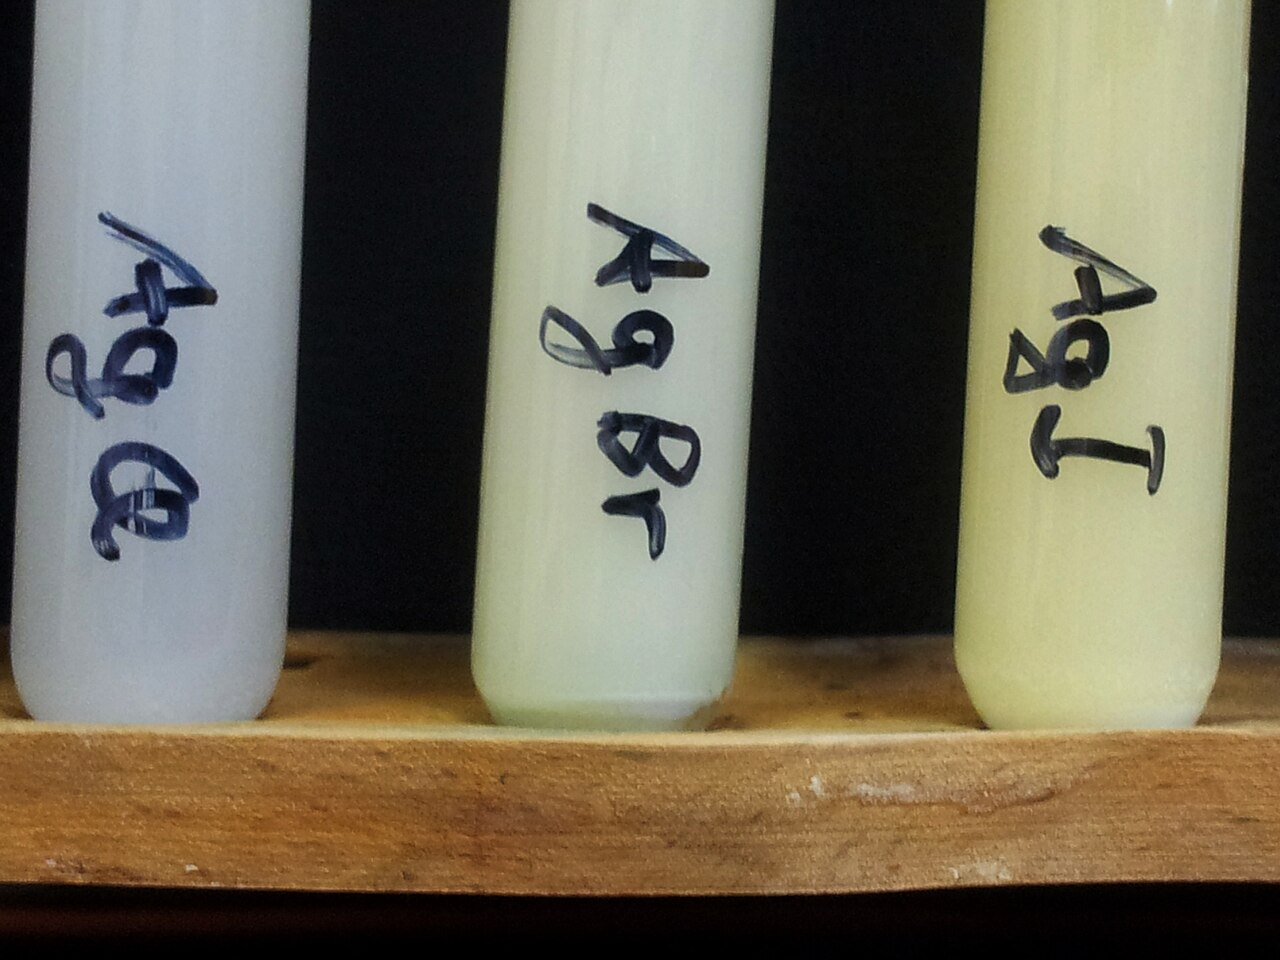
\includegraphics[width=0.6\linewidth]{images/book2/silver-halides.jpg}

{\small Precipitados de cloruro de plata (blanco), bromuro de plata (crema)
y yoduro de plata (amarillo pálido). Fotografía de Rrausch1974, CC BY-SA
3.0, Wikimedia Commons.}
\end{omfigure}

\section{Solubilidad}

\begin{definition}[Solubilidad]\label{def:b1:precipitation:solubility}
La \emph{solubilidad}\index{solubilidad} $s$ de un sólido en una
disolución dada es la cantidad de sólido que se disuelve en un litro de
esa disolución hasta la saturación (en \unit{mol/L}); multiplicada por la
masa molar, es la solubilidad en masa, en \unit{g/L}. Depende de la
temperatura y de la composición de la disolución.
\end{definition}

\begin{proposition}[Solubilidad a partir del producto de solubilidad]\label{prop:b1:precipitation:s-of-ks}
En agua pura, si los iones no intervienen en ninguna otra reacción,
\[
  \mathrm{MX}:\ s = \sqrt{K_s}, \qquad
  \mathrm{MX_2}\ \text{o}\ \mathrm{M_2X}:\ s = \left(\frac{K_s}{4}\right)^{1/3},
  \qquad
  \mathrm{M}_a\mathrm{X}_b:\ s = \left(\frac{K_s}{a^a b^b}\right)^{1/(a+b)} .
\]
\end{proposition}

\begin{proof}
Cuando se disuelven $s$ mol de sólido por litro, $[\mathrm{M}^{m+}] = as$
y $[\mathrm{X}^{x-}] = bs$, de modo que en la saturación $K_s = (as)^a(bs)^b =
a^a b^b s^{a+b}$. Para MX, $a = b = 1$; para \ce{MX2}, $1^1 2^2 = 4$, y lo
mismo para \ce{M2X}.
\end{proof}

\begin{example}[Cloruro de plata y cromato de plata]\label{ex:b1:precipitation:agcl-ag2cro4}
Cloruro de plata: $s = 10^{-9.75/2} = \qty{1.3e-5}{mol/L}$, es decir,
\qty{1.9}{mg/L} con $M = \qty{143.4}{g/mol}$. Cromato de plata
\ce{Ag2CrO4}
($\mathrm{p}K_s = 11.95$): $s = (10^{-11.95}/4)^{1/3} =
\qty{6.6e-5}{mol/L}$. El cromato tiene la $K_s$ más pequeña y, sin
embargo, es cinco veces más soluble. Los \omterm{def:b1:precipitation:solubility-product}{productos de solubilidad} solo
pueden compararse directamente entre sólidos del mismo tipo de fórmula.
\end{example}

\begin{remark}
Las fórmulas suponen que los iones están libres. En agua pura, el ion
cromato es una \omterm{def:b1:predominant-reaction:strong-acid}{base débil} y el ion plata no está complejado por nada, de
modo que el resultado para el cromato de plata es casi correcto; para un
carbonato, un sulfuro o un hidróxido, las propiedades básicas del anión
importan y hace falta la sección siguiente. A fuerza iónica elevada, las
\omterm{def:b1:extent-q-and-k:activity}{actividades} también se alejan de las concentraciones, una corrección que
se deja para el volumen del segundo año.
\end{remark}

\section{Efectos del ion común y del pH}

\begin{definition}[Efecto del ion común]\label{def:b1:precipitation:common-ion}
El \emph{efecto del ion común}\index{efecto del ion comun@efecto del ion común} es la disminución de
la \omterm{def:b1:precipitation:solubility}{solubilidad} de un sólido en una disolución que ya contiene uno de sus
iones.
\end{definition}

\begin{proposition}[Solubilidad con un ion común]\label{prop:b1:precipitation:common-ion}
Sea MX que se disuelve en una disolución en la que ya $[\mathrm{X}^-] = c$,
con $c \gg \sqrt{K_s}$. Entonces, $s \approx K_s/c$, mucho menor que en
agua pura. Para \ce{MX2} en una disolución que contiene \ce{M^2+} a $c$,
$s \approx \frac12\sqrt{K_s/c}$.
\end{proposition}

\begin{proof}
En la saturación, $[\mathrm{M}^+] = s$ y $[\mathrm{X}^-] = c + s$, de modo
que $s(c + s) = K_s$. Si $s \ll c$, $s = K_s/c$; la hipótesis se cumple,
pues $K_s/c \ll c$ cuando $c^2 \gg K_s$. Para \ce{MX2}, $[\ce{X-}] = 2s$ y
$[\mathrm{M}^{2+}] = c + s \approx c$, de modo que $c\,(2s)^2 = K_s$.
\end{proof}

Cloruro de plata en cloruro de sodio de \qty{0.10}{mol/L}:
$s = 10^{-9.75}/0.10
= \qty{1.8e-9}{mol/L}$, siete mil veces menos que en agua. Por eso un
precipitado se lava con una disolución diluida de un ion común y no con
agua pura: pierde menos de sí mismo.

Cuando el anión del sólido es una base, el ácido lo saca del equilibrio de
disolución y la \omterm{def:b1:precipitation:solubility}{solubilidad} aumenta. Para el carbonato de calcio en
medio ácido,
\[
  \ce{CaCO3(s) + H3O+ <=> Ca^2+ + HCO3- + H2O}, \qquad
  K = \frac{K_s}{K_{a2}} = 10^{-8.30 + 10.33} = 10^{2.03} ,
\]
una reacción favorecida: el vinagre o el ácido clorhídrico disuelven la
caliza, y el dióxido de carbono que forma la reacción posterior del
\ce{HCO3-} produce la conocida efervescencia.
% ledger: dfg:HCO3-_ao (pKa2 of carbonic acid, ch. 10)

\begin{proposition}[Solubilidad de un hidróxido en función del pH]\label{prop:b1:precipitation:hydroxide-ph}
En una disolución tamponada a un pH dado, la concentración de \ce{M^{n+}}
en equilibrio con el hidróxido \ce{M(OH)_n} cumple
\[
  \log[\mathrm{M}^{n+}] = -\mathrm{p}K_s + n\,(\mathrm{p}K_e - \mathrm{pH}) ,
\]
una recta de pendiente $-n$ frente al pH. Si el ion no forma ningún
complejo, es la \omterm{def:b1:precipitation:solubility}{solubilidad} del hidróxido.
\end{proposition}

\begin{proof}
$K_s = [\mathrm{M}^{n+}][\ce{OH-}]^n$ y $[\ce{OH-}] = K_e/[\ce{H3O+}]$, de
modo que $\log[\mathrm{M}^{n+}] = \log K_s - n\log[\ce{OH-}] = -\mathrm{p}K_s -
n(\mathrm{pH} - \mathrm{p}K_e)$.
\end{proof}

Cada unidad de pH divide por mil la \omterm{def:b1:precipitation:solubility}{solubilidad} del hidróxido de
hierro(III), y por cien la del hidróxido de cinc. Los hidróxidos se
precipitan, y se vuelven a disolver, cambiando el pH.

\begin{example}[Disolver carbonato de calcio con dióxido de carbono]\label{ex:b1:precipitation:cave}
El agua que contiene dióxido de carbono disuelto disuelve la calcita:
\[
  \ce{CaCO3(s) + CO2(aq) + H2O <=> Ca^2+ + 2HCO3-}, \qquad
  K = \frac{K_s K_{a1}}{K_{a2}} = 10^{-8.30 - 6.37 + 10.33} = 10^{-4.34} ,
\]
constante que se obtiene sumando la disolución del carbonato, la primera
acidez del dióxido de carbono y la inversa de la segunda. Cuanto más
dióxido de carbono, más carbonato de calcio se disuelve. El aire del
suelo suele ser mucho más rico en dióxido de carbono que el de una cueva;
el agua que ha atravesado el suelo y llega al techo de la cueva pierde
dióxido de carbono, y la calcita se deposita
(\cref{exo:b1:precipitation:10}).
\end{example}

\section{Dominios de existencia y precipitación selectiva}\label{sec:b1:precipitation:domains}

\begin{definition}[Dominio de existencia]\label{def:b1:precipitation:existence-domain}
Para un sólido y una concentración total dada $c$ de uno de sus iones, el
\emph{dominio de existencia}\index{dominio de existencia} del sólido es el
intervalo de la variable (pX, pM o pH) en el que el sólido está presente
en el equilibrio. Su frontera es el valor en el que aparece el primer
grano de sólido, cuando $Q_s = K_s$ con el ion todavía a la concentración
$c$.
\end{definition}

\begin{method}[Trazar un diagrama de existencia]\label{met:b1:precipitation:existence-domain}
\begin{enumerate}
  \item Se fija la concentración total $c$ del ion que no está en el eje
        (por ejemplo, $[\ce{Ag+}]_{\mathrm{tot}} = c$ en un eje de pCl).
  \item Se escribe $K_s$ al comienzo de la precipitación, con ese ion
        todavía a $c$, y se despeja la variable del eje.
  \item El sólido existe del lado en el que el otro ion está concentrado:
        pCl pequeño (mucho cloruro), pAg pequeño o pH alto para un
        hidróxido.
  \item No se marca ningún dominio para el propio ion: está presente en
        todas partes, a $c$ fuera del dominio del sólido y por debajo de
        $c$ dentro de él.
\end{enumerate}
\end{method}

Para el cloruro de plata con $c = [\ce{Ag+}]_{\mathrm{tot}} = 10^{-2}$: la
precipitación empieza cuando $[\ce{Cl-}] = K_s/c = 10^{-7.75}$, de modo
que el sólido existe para $\mathrm{pCl} < 7.75$. Para el yoduro de plata,
la frontera está en
$\mathrm{pI} = 16.07 - 2 = 14.07$, como se dibuja abajo.

\begin{omfigure}
\begin{tikzpicture}[font=\small, >={Stealth}, x=0.62cm]
  \fill[omDef!18] (0,0.12) rectangle (7.75,0.6);
  \draw[->, thick] (0,0) -- (17.2,0) node[right] {pCl o pI};
  \foreach \x in {0,2,4,6,8,10,12,14,16}
    \draw (\x,0.08) -- (\x,-0.08) node[below] {\x};
  \draw[omDef, thick] (7.75,-0.5) -- (7.75,0.9);
  \node[omDef] at (3.9,0.36) {existe \ce{AgCl(s)}};
  \node[omDef, above] at (7.75,0.9) {7.75};
  \node[anchor=west] at (8.0,0.36) {sin sólido: \ce{Ag+} a $10^{-2}$ mol/L};
  % AgI below
  \begin{scope}[yshift=-1.9cm]
  \fill[omProp!20] (0,0.12) rectangle (14.07,0.6);
  \draw[->, thick] (0,0) -- (17.2,0);
  \foreach \x in {0,2,4,6,8,10,12,14,16}
    \draw (\x,0.08) -- (\x,-0.08) node[below] {\x};
  \draw[omProp, thick] (14.07,-0.5) -- (14.07,0.9);
  \node[omProp] at (7.0,0.36) {existe \ce{AgI(s)}};
  \node[omProp, above] at (14.07,0.9) {14.07};
  \end{scope}
\end{tikzpicture}

{\small \omterm{def:b1:precipitation:existence-domain}{Dominios de existencia} del cloruro de plata (en un eje de pCl,
arriba) y del yoduro de plata (en un eje de pI, abajo) para una
concentración total de plata de \qty{1.0e-2}{mol/L}. El yoduro precipita
la plata a concentraciones un millón de veces menores que el cloruro.}
\end{omfigure}

\begin{method}[Precipitación selectiva]\label{met:b1:precipitation:selective}
Para separar dos iones que precipitan con el mismo reactivo:
\begin{enumerate}
  \item se calcula, para cada ion a su concentración, la concentración de
        reactivo (o el pH) a la que su sólido empieza a formarse; el
        menor precipita primero;
  \item se calcula la concentración del primer ion que queda en
        disolución cuando el segundo empieza a precipitar;
  \item la separación es aceptable si esa concentración es una fracción
        suficientemente pequeña de la inicial --- típicamente un
        \qty{0.1}{\percent} ---, y entonces se detiene la adición de
        reactivo entre los dos umbrales.
\end{enumerate}
\end{method}

\begin{example}[Yoduro y cloruro]\label{ex:b1:precipitation:i-cl}
Una disolución contiene iones yoduro y cloruro, ambos a
\qty{1.0e-2}{mol/L}; se añade nitrato de plata gota a gota, sin
dilución. El yoduro de plata empieza a formarse cuando
$[\ce{Ag+}] = 10^{-16.07 + 2} =
10^{-14.07}$, y el cloruro de plata, cuando vale $10^{-9.75 + 2} = 10^{-7.75}$:
el yoduro precipita primero. Cuando aparece el cloruro de plata,
$[\ce{I-}] = 10^{-16.07}/10^{-7.75} = 10^{-8.32} = \qty{4.8e-9}{mol/L}$,
una fracción $5 \times 10^{-7}$ del yoduro: la separación es completa.
\end{example}

Los hidróxidos se separan del mismo modo, con el pH como variable. El
gráfico de abajo muestra, para seis iones a \qty{0.010}{mol/L}, el pH en
el que aparece el hidróxido y el pH en el que ha precipitado el
\qty{99.9}{\percent} del ion. El hierro(III) y el aluminio se eliminan en
agua ácida; el cinc y el hierro(II), cerca de la neutralidad; el magnesio,
hacia pH 10, y el calcio, solo en agua muy básica.

\begin{omfigure}
\begin{tikzpicture}
\begin{axis}[
  width=0.82\linewidth, height=5.4cm, xmin=0, xmax=14, ymin=0.4, ymax=6.6,
  axis x line=bottom, axis y line=left, xlabel={pH},
  xtick={0,2,4,6,8,10,12,14}, ytick={1,2,3,4,5,6},
  yticklabels={\ce{Fe^3+}, \ce{Al^3+}, \ce{Zn^2+}, \ce{Fe^2+}, \ce{Mg^2+}, \ce{Ca^2+}},
  y dir=reverse, axis line style={-},
  tick label style={font=\small}, label style={font=\small}]
\addplot[draw=none, omDef!35,
  error bars/.cd, x dir=plus, x explicit,
  error bar style={line width=7pt, omDef!35}, error mark=none]
  table[x=start, y=row, x error expr=14-\thisrow{start}] {figdata/out/bachelor-1-solubility-ph-thresholds.dat};
\addplot[draw=none, omDef,
  error bars/.cd, x dir=plus, x explicit,
  error bar style={line width=7pt, omDef}, error mark=none]
  table[x=start, y=row, x error expr=\thisrow{end}-\thisrow{start}] {figdata/out/bachelor-1-solubility-ph-thresholds.dat};
\end{axis}
\end{tikzpicture}

{\small Precipitación de los hidróxidos a partir de disoluciones de
\qty{0.010}{mol/L} de cada ion. La barra oscura va desde el primer grano
de hidróxido hasta el pH en el que ha precipitado el
\qty{99.9}{\percent} del ion (una unidad de pH de ancho para un ion
trivalente, y una y media para uno divalente); la barra clara es el resto
del \omterm{def:b1:precipitation:existence-domain}{dominio de existencia} del hidróxido. No se muestra la redisolución
anfótera de los hidróxidos de cinc y de aluminio a pH alto
(\cref{sec:b1:precipitation:amphoteric}).}
\end{omfigure}

\section{Hidróxidos anfóteros}\label{sec:b1:precipitation:amphoteric}

Se añade hidróxido de sodio gota a gota a una disolución de sulfato de
cinc: se forma un precipitado blanco de hidróxido de cinc que, con un
exceso de hidróxido, vuelve a disolverse. El hidróxido de aluminio hace
lo mismo; los hidróxidos de hierro(III) y de magnesio, no.

\begin{definition}[Hidróxido anfótero]\label{def:b1:precipitation:amphoteric-hydroxide}
Un hidróxido es un \emph{hidróxido anfótero}\index{hidroxido anfotero@hidróxido anfótero}
si se disuelve tanto en ácido, como catión, como en exceso de base, como
anión complejo hidroxo:
\[
  \ce{Zn(OH)2(s) + 2H3O+ -> Zn^2+ + 4H2O}, \qquad
  \ce{Zn(OH)2(s) + 2OH- -> Zn(OH)4^2-} .
\]
\end{definition}

El anión complejo \ce{Zn(OH)4^2-} (tetrahidroxocincato) se caracteriza
por su constante de formación $\beta_4 = [\ce{Zn(OH)4^2-}]/([\ce{Zn^2+}][\ce{OH-}]^4)
= 10^{14.45}$; los complejos y sus constantes son el objeto del
\cref{ch:b1:complexation}.

\begin{proposition}[Solubilidad de un hidróxido anfótero]\label{prop:b1:precipitation:amphoteric}
Si el cinc solo está en disolución como \ce{Zn^2+} y \ce{Zn(OH)4^2-}, la
\omterm{def:b1:precipitation:solubility}{solubilidad} del hidróxido de cinc es
\[
  s = [\ce{Zn^2+}] + [\ce{Zn(OH)4^2-}] = \frac{K_s}{[\ce{OH-}]^2} + K\,[\ce{OH-}]^2,
  \qquad K = \beta_4 K_s = 10^{-1.93} .
\]
En $\log s$ frente al pH, sigue una recta de pendiente $-2$ a pH bajo y una
recta de pendiente $+2$ a pH alto. Es mínima cuando
$[\ce{OH-}]^4 = K_s/K = 1/\beta_4$, es decir, en $\mathrm{pH} =
\mathrm{p}K_e - \frac14\log\beta_4$, donde $s_{\min} = 2\sqrt{K_s K}$.
\end{proposition}

\begin{proof}
En la saturación, $[\ce{Zn^2+}] = K_s/[\ce{OH-}]^2$; la concentración del
complejo es entonces
$[\ce{Zn(OH)4^2-}] = \beta_4[\ce{Zn^2+}][\ce{OH-}]^4 = \beta_4 K_s
[\ce{OH-}]^2$. Con $w = [\ce{OH-}]^2$, $s(w) = K_s/w + Kw$ tiene por
derivada $-K_s/w^2 + K$, que se anula en $w = \sqrt{K_s/K}$, donde
$s = 2\sqrt{K_s K}$. A
pH bajo domina el primer término y $\log s = \log K_s - 2\log[\ce{OH-}]$
(pendiente $-2$ en pH); a pH alto, el segundo, $\log s = \log K + 2\log[\ce{OH-}]$
(pendiente $+2$).
\end{proof}

Con los valores anteriores, el mínimo está en
$\mathrm{pH} = 14.00 - 14.45/4
= 10.39$ y $s_{\min} = 2 \times 10^{-(16.38 + 1.93)/2} =
\qty{1.4e-9}{mol/L}$
(figura de abajo). El mínimo real es mucho más alto: el cinc también forma
\ce{ZnOH+}, \ce{Zn(OH)3-} y, sobre todo, una especie disuelta sin carga,
\ce{Zn(OH)2(aq)}, cuya concentración en equilibrio con el sólido no
depende del pH. El cálculo completo, con las mismas tablas, sitúa el suelo
hacia $10^{-5.6}$~mol/L. Un modelo de dos especies da las pendientes y el
orden de los umbrales; cerca del mínimo, todas las especies cuentan.

\begin{omfigure}
\begin{tikzpicture}
\begin{axis}[name=zn,
  width=0.46\linewidth, height=5.6cm, xmin=6, xmax=14, ymin=-10, ymax=0,
  axis x line=bottom, axis y line=left, xlabel={pH}, ylabel={$\log s$},
  xtick={6,8,10,12,14}, ytick={-10,-8,-6,-4,-2,0},
  tick label style={font=\small}, label style={font=\small}]
\addplot[omProp, dashed, thick] table[x=pH, y=full] {figdata/out/bachelor-1-solubility-ph-zinc.dat};
\addplot[omDef, very thick] table[x=pH, y=model] {figdata/out/bachelor-1-solubility-ph-zinc.dat};
\node[font=\small, anchor=west] at (axis cs:7.0,-1.0) {\ce{Zn^2+}};
\node[font=\small, anchor=east] at (axis cs:13.8,-1.1) {\ce{Zn(OH)4^2-}};
\node[font=\small, omProp, anchor=south] at (axis cs:10.4,-5.5) {todas las especies};
\node[font=\small, anchor=north] at (axis cs:10.2,-0.4) {cinc};
\end{axis}
\begin{axis}[at={(zn.east)}, anchor=west, xshift=1.8cm,
  width=0.46\linewidth, height=5.6cm, xmin=2, xmax=14, ymin=-10, ymax=0,
  axis x line=bottom, axis y line=left, xlabel={pH}, ylabel={$\log s$},
  xtick={2,4,6,8,10,12,14}, ytick={-10,-8,-6,-4,-2,0},
  tick label style={font=\small}, label style={font=\small}]
\addplot[omDef, very thick] table[x=pH, y=model] {figdata/out/bachelor-1-solubility-ph-aluminium.dat};
\node[font=\small, anchor=west] at (axis cs:3.4,-0.8) {\ce{Al^3+}};
\node[font=\small, anchor=east] at (axis cs:13.8,-0.6) {\ce{Al(OH)4-}};
\node[font=\small, anchor=north] at (axis cs:8.6,-0.4) {aluminio};
\end{axis}
\end{tikzpicture}

{\small \omterm{def:b1:precipitation:solubility}{Solubilidad} del hidróxido de cinc (izquierda) y del hidróxido de
aluminio, gibbsita (derecha), en función del pH, según el modelo de dos
especies (líneas continuas): pendientes $-2$ y $+2$ para el cinc, $-3$ y
$+1$ para el aluminio. Para el cinc, la curva discontinua incluye todas
las especies hidroxo, y el \ce{Zn(OH)2(aq)} sin carga fija un suelo.}
\end{omfigure}

Para el aluminio, el hidróxido es \ce{Al(OH)3} y el complejo,
\ce{Al(OH)4-}, de modo que $\ce{Al(OH)3(s) + OH- <=> Al(OH)4-}$ con
$K = \beta_4 K_s = 10^{33.52
- 34.75} = 10^{-1.23}$ y pendientes $-3$ y $+1$. La diferencia entre el
aluminio y el hierro(III) --- uno anfótero, el otro no --- se aprovecha en
la industria para separarlos: el hidróxido de sodio caliente disuelve el
aluminio de la bauxita y deja atrás los óxidos de hierro
(\cref{exo:b1:precipitation:12}).

\section{Ejercicios}

\begin{exercise}[$\star$]\label{exo:b1:precipitation:1}
Escríbanse la ecuación de disolución y la expresión de $K_s$ de
\ce{BaSO4}, \ce{CaF2}, \ce{Ag2CrO4} y \ce{Fe(OH)3}. Dese $K_s$ en
potencias de diez a partir de la tabla de la \cref{sec:b1:precipitation:product},
y el $\mathrm{p}K_s$ de un sólido de $K_s = \num{2.0e-13}$.
\end{exercise}

\begin{exercise}[$\star$]\label{exo:b1:precipitation:2}
Calcúlese la \omterm{def:b1:precipitation:solubility}{solubilidad} del bromuro de plata en agua pura en
\unit{mol/L} y en \unit{mg/L} ($M = \qty{187.8}{g/mol}$).
\end{exercise}

\begin{exercise}[$\star$]\label{exo:b1:precipitation:3}
Se mezclan \qty{50}{mL} de cloruro de bario de \qty{2.0e-3}{mol/L} con
\qty{50}{mL} de sulfato de sodio de \qty{2.0e-4}{mol/L}. ¿Precipita el
sulfato de bario? La misma pregunta con sulfato de sodio de
\qty{2.0e-7}{mol/L}.
\end{exercise}

\begin{exercise}[$\star$]\label{exo:b1:precipitation:4}
Calcúlese la \omterm{def:b1:precipitation:solubility}{solubilidad} del sulfato de bario en agua pura y, después,
en una disolución de sulfato de sodio de \qty{0.010}{mol/L}. ¿En qué
factor ha cambiado?
\end{exercise}

\begin{exercise}[$\star\star$]\label{exo:b1:precipitation:5}
Calcúlese la \omterm{def:b1:precipitation:solubility}{solubilidad} del fluoruro de calcio en agua pura
(\unit{mol/L} y
\unit{mg/L}, $M = \qty{78.1}{g/mol}$) y, después, en una disolución de
cloruro de calcio de \qty{0.10}{mol/L}. Compruébese la aproximación
realizada.
\end{exercise}

\begin{exercise}[$\star\star$]\label{exo:b1:precipitation:6}
Una disolución contiene iones magnesio a \qty{0.050}{mol/L}. ¿A qué pH
empieza a precipitar el hidróxido de magnesio? ¿A qué pH ha precipitado
el \qty{99}{\percent} del magnesio? Dibújese el \omterm{def:b1:precipitation:existence-domain}{dominio de existencia} de
\ce{Mg(OH)2} en un eje de pH.
\end{exercise}

\begin{exercise}[$\star\star$]\label{exo:b1:precipitation:7}
Una disolución contiene iones bromuro y cloruro, ambos a
\qty{1.0e-2}{mol/L}. Se añade nitrato de plata sin dilución. ¿Qué
precipitado aparece primero? ¿Qué fracción del primer ion queda aún en
disolución cuando aparece el segundo sólido? ¿Es aceptable la
separación?
\end{exercise}

\begin{exercise}[$\star\star$]\label{exo:b1:precipitation:8}
La valoración de Mohr del cloruro con iones plata usa iones cromato como
indicador: el cromato de plata, rojo, solo debe aparecer cuando ya ha
precipitado casi todo el cloruro. El cloruro está a \qty{0.050}{mol/L} y
el cromato a \qty{5.0e-3}{mol/L}; se desprecia la dilución. Calcúlense
$[\ce{Ag+}]$ cuando empieza a formarse el cromato de plata y la fracción
de cloruro que sigue en disolución en ese momento.
\end{exercise}

\begin{exercise}[$\star\star$]\label{exo:b1:precipitation:9}
Se agita carbonato de calcio con una disolución mantenida a pH 8.30 por
un tampón, en la que el hidrogenocarbonato es con mucho la especie
carbonatada principal. Demuéstrese que
$[\ce{Ca^2+}][\ce{HCO3-}] = K_s\,10^{\mathrm{p}K_{a2} - \mathrm{pH}}$ y
calcúlese la \omterm{def:b1:precipitation:solubility}{solubilidad}, suponiendo que todo el carbonato disuelto
permanece como \ce{HCO3-} ($\mathrm{p}K_{a2} = 10.33$).
\end{exercise}

\begin{exercise}[$\star\star\star$]\label{exo:b1:precipitation:10}
Las cuevas calizas. La \omterm{def:b1:precipitation:solubility}{solubilidad} del dióxido de carbono sigue
\ce{CO2(g) <=> CO2(aq)} con $\log K_H = -1.47$ ($K_H =
[\ce{CO2(aq)}]/p(\ce{CO2})$, con la presión en bar).
\begin{enumerate}
  \item Combínese $K_H$ con la constante del
        \cref{ex:b1:precipitation:cave} para obtener la constante de
        \ce{CaCO3(s) + CO2(g) + H2O <=> Ca^2+ + 2HCO3-}.
  \item Demuéstrese que la \omterm{def:b1:precipitation:solubility}{solubilidad} de la calcita es $s = (K'p/4)^{1/3}$
        y calcúlese en agua que se ha equilibrado con el aire del suelo, a
        $p(\ce{CO2}) = \qty{0.010}{bar}$, y después con el aire exterior,
        \qty{4.26e-4}{bar}. Dense ambas en \unit{mg/L} de \ce{CaCO3}
        ($M = \qty{100.1}{g/mol}$).
  \item Explíquese el crecimiento de una estalactita.
\end{enumerate}
\end{exercise}

\begin{exercise}[$\star\star\star$]\label{exo:b1:precipitation:11}
Se lleva a pH creciente una disolución de cinc de \qty{1.0e-2}{mol/L}, en
la que el cinc solo está presente como \ce{Zn^2+} y \ce{Zn(OH)4^2-}.
\begin{enumerate}
  \item ¿Entre qué valores de pH está presente el hidróxido de cinc?
  \item Hállense el pH de \omterm{def:b1:precipitation:solubility}{solubilidad} mínima y la \omterm{def:b1:precipitation:solubility}{solubilidad} mínima.
  \item Esbócese $\log s$ frente al pH e indíquense las pendientes.
\end{enumerate}
\end{exercise}

\begin{exercise}[$\star\star\star$]\label{exo:b1:precipitation:12}
Una disolución contiene iones aluminio y hierro(III), cada uno a
\qty{1.0e-3}{mol/L}. Se añade hidróxido de sodio en exceso.
\begin{enumerate}
  \item ¿Por encima de qué pH está todo el aluminio disuelto como
        \ce{Al(OH)4-}?
  \item ¿Cuál es entonces la concentración de \ce{Fe^3+}? Conclúyase sobre
        la separación.
  \item Explíquese por qué la separación fallaría con magnesio en lugar de
        aluminio.
\end{enumerate}
\end{exercise}

\section{Problema: depurar un efluente minero}

\begin{problem}[{Problema de fin de semana --- umbrales de precipitación de
tres hidróxidos, el complejo hidroxo del hierro(III), la recuperación del
cinc y su redisolución anfótera, y la ventana de pH para eliminar el
hierro(III) sin perder el cinc(II)}]
\label{pb:b1:precipitation:1}
El agua que drena de una antigua mina metálica es ácida (pH 2.0) y
contiene hierro(III) a \qty{1.0e-3}{mol/L}, cinc(II) a
\qty{5.0e-3}{mol/L} y magnesio a \qty{2.0e-2}{mol/L}. La planta eleva el
pH paso a paso para eliminar el hierro como lodo de desecho, recuperar
después el cinc como hidróxido y dejar en el agua el magnesio, inofensivo.
Datos a \qty{25}{\celsius}: $\mathrm{p}K_s$ de \ce{Fe(OH)3} 38.55,
\ce{Zn(OH)2}
16.38, \ce{Mg(OH)2} 11.25; $\log\beta_4(\ce{Zn(OH)4^2-}) = 14.45$;
$\log\beta_1(\ce{FeOH^2+}) = 11.82$; $\mathrm{p}K_e = 14.00$; masas
molares: \ce{Fe(OH)3} \qty{106.8}{g/mol}, \ce{Zn(OH)2} \qty{99.4}{g/mol}.

\medskip
\noindent\textbf{Parte I --- ¿Qué hidróxido primero?}
\begin{enumerate}
  \item Escríbanse los equilibrios de disolución de los tres hidróxidos y
        sus $K_s$.
  \item Explíquese por qué los tres $\mathrm{p}K_s$ por sí solos no dicen
        qué hidróxido precipita primero.
  \item Demuéstrese que \ce{M(OH)_n} empieza a precipitar a partir de una
        disolución de \ce{M^{n+}} a $c$ en $\mathrm{pH} = \mathrm{p}K_e -
        \frac1n(\mathrm{p}K_s + \log c)$.
  \item Calcúlese ese pH para el hierro(III).
  \item Calcúlese para el cinc.
  \item Calcúlese para el magnesio.
  \item Dese el orden de precipitación a medida que sube el pH. ¿Hay algo
        precipitado en el efluente cuando sale de la mina?
\end{enumerate}

\medskip
\noindent\textbf{Parte II --- Eliminar el hierro: primera estimación.}
\begin{enumerate}[resume]
  \item La planta quiere sacar del agua el \qty{99.9}{\percent} del
        hierro. ¿Qué concentración de hierro disuelto permite eso?
  \item Despreciando cualquier complejo, ¿a qué pH se alcanza?
  \item Demuéstrese que, en el \omterm{def:b1:precipitation:existence-domain}{dominio de existencia} de \ce{Fe(OH)3},
        $\log[\ce{Fe^3+}]$ disminuye 3 unidades por unidad de pH.
  \item ¿Hasta qué pH permanece el cinc íntegramente en disolución?
  \item Dese la primera estimación de la ventana de pH en la que se
        elimina el hierro mientras el cinc permanece.
\end{enumerate}

\medskip
\noindent\textbf{Parte III --- El complejo hidroxo del hierro(III).}
\begin{enumerate}[resume]
  \item Escríbanse la formación de \ce{FeOH^2+} a partir de \ce{Fe^3+} y
        \ce{OH-} y su constante.
  \item Dibújese el \omterm{def:b1:predominant-reaction:predominance}{diagrama de predominio} de \ce{Fe^3+} y \ce{FeOH^2+} en
        función del pH.
  \item Al pH hallado en la pregunta 9, calcúlese
        $[\ce{FeOH^2+}]/[\ce{Fe^3+}]$. ¿Era segura la primera estimación?
  \item Exprésese el hierro disuelto total, $[\ce{Fe^3+}] + [\ce{FeOH^2+}]$,
        en equilibrio con \ce{Fe(OH)3} en función del pH.
  \item Demuéstrese que, donde predomina \ce{FeOH^2+}, su logaritmo
        disminuye 2 unidades por unidad de pH.
  \item Hállese el pH al que el hierro disuelto total baja al valor de la
        pregunta 8.
\end{enumerate}

\medskip
\noindent\textbf{Parte IV --- Recuperar el cinc.}
\begin{enumerate}[resume]
  \item Una vez filtrado el lodo de hierro, se vuelve a elevar el pH. ¿A
        qué pH ha precipitado el \qty{99}{\percent} del cinc? ¿Se forma
        hidróxido de magnesio a ese pH?
  \item Escríbase la reacción del hidróxido de cinc con un exceso de iones
        hidróxido y calcúlese su constante.
  \item ¿Por encima de qué pH volvería a estar todo el cinc en disolución?
        ¿Qué significa esto para el operador?
  \item Calcúlese la masa de lodo de hidróxido de hierro(III) eliminada
        por metro cúbico de efluente.
  \item Calcúlese la masa de hidróxido de cinc recuperada por metro cúbico
        al pH de la pregunta 19.
  \item ¿Por qué hay que eliminar el hierro antes que el cinc, y no ambos
        juntos?
  \item Dese la ventana de pH, con dos decimales, en la que el hierro(III)
        se elimina en un \qty{99.9}{\percent} mientras el cinc(II)
        permanece íntegramente en disolución.
\end{enumerate}
\end{problem}
